% !TeX root = ../main.tex
% Add the above to each chapter to make compiling the PDF easier in some editors.
\chapter{Related Work}\label{chapter:related-work}

\section{Classification of location data usage according to acceptable delay}
In order to review existing approaches and research, we classify location aware services by the acceptable delay of the location information being available. Similar to the classification made by \parencite{hoh2005protecting}, we define three categories:
\begin{enumerate}
  \item Almost no delay tolerance: e.g. an application showing a pop-up about a nearby venue e.g. a coffe shop when a pedestrian passes by.
  \item Some delay tolerance e.g. one minute: An application e.g. google maps derives the information of congested traffic from devices reporting their GPS data which show lower than usually on the respective road. As congestions worth reporting last longer than one minute, some delay in the device's information reaching the server is acceptable.
  \item Significant delay tolerance of hours, days or even weeks: For historical and statistical use of location data e.g. to find out about popular visiting times of a venue, almost any delay is acceptable.
\end{enumerate}
Some research deals with case one where almost no delay tolerance is acceptable \parencite{location-privacy, mix-zones}. \parencite{casper} proposes a solution where not the exact location is send to a server but the rough region of the user. The server then sends a list of all possible matches like e.g. venues in this area to the client. Locally, this list is then matched with the exact location in order to fulfill the aim of the respective application.
Most research though investigates user's privacy in case 3 where the delay of the data being available for processing is not an issue \parencite{krumm, cellphone, privacy-home-work-pairs, twitter}. In the following, we will concentrate on this case as well.
%Our research targets case 3 in which a significant delay is acceptable.
%review research tackling location privacy in case 3 and 2 and then briefly point out the findings for case 1.

%\subsection{What has been achieved so far}

%Most existing approaches focus on publishing location data where a huge delay is acceptable as can be seen in the following table: TODO [create table].

\section{Privacy problems arising from location data}
\subsection{Risk of privacy intrusion through theft of central databases}
Centralized databases containing raw location data expose users to a privacy risk (through theft) \parencite{iot, hoh2006enhancing}. \parencite{p2p-android} proposes the use of P2P over WIFI and Bluetooth to decrease the need of central instances. A decentralized analysis approach and it's implications for data privacy is also investigated by \parencite{iot} as an alternative to cloud-based IoT.
\parencite{crowdsourcing} proposes an approach in which raw data is hidden from the central instance but still aggregated data can be obtained by using encryption methods. Raw data is encrypted using a modified approach of public-private key-pair cryptography in which the sum of two encrypted messages can be decrypted to the sum of the encrypted messages. Furthermore, only a number of messages above a certain threshold can be encrypted this way using the different encryption shares. 
%While this approach is close to our work in general, we propose a more general and flexible setup.
Another approach by \parencite{hoh2006enhancing} also uses encryption in combination with a middleware. The server storing the data and the participant (e.g. a vehicle) share a symmetric key which is stored securely in the vehicle. The middleware ensures authentication of the participant, and forwards the location to the central server without giving away the vehicle's identity. Nevertheless, several research as e.g. \parencite{krumm, twitter, cellphone} have shown that it is easy to infer identity from such datasets. 
%Even though they solve the problem of user authentication, it seems hardly feasable as the symmetric key has to be pre-installed on every participating device.

\subsection{Inference attacks on published anonymized data}
%\subsection{Inferring home and work location from consecutive data samples}
Research has shown, that from a location data set that is pseudonymous, i.e. the identifiers have been stripped off or the data-set has been anonymized in another way, it is possible to infer the home location of single users through so-called inference attacks \parencite{krumm, cellphone, privacy-home-work-pairs, hoh2006enhancing, twitter} and also the work location with a slightly lower probability \parencite{cellphone, privacy-home-work-pairs}. The same problem arises when using data collected through crowdsourcing \parencite{crowdsourcing}.
These home locations or home-work location pairs can then be used to look up the corresponding user's identity e.g. by combining it with publicly available information. One possibility is to reverse code GPS coordinates to addresses and then e.g. search for entries in telephone books to infer the user's identity from it's home location \parencite{krumm, privacy-home-work-pairs, hoh2006enhancing}. Especially in suburban areas this is quite successful as usually one house can be mapped to only one person or family. This identity can then be linked to other sensitive data, e.g. locations visited by the identified user. The same problem also arises in the area of IoT \parencite{iot, hoh2006enhancing}.

\section{Countermeasures to prevent inference attacks}
In general, the problem can be solved by providing k-anonymity for the data-set \parencite{k-anonymity}. A data-set is k-anonymous, if querying for an identifier in this data-set always returns a result set of at least k entries.
In order to achieve this, several approaches have been investigated. 
\parencite{krumm} propose spatial cloaking. K-anonymity is achieved by dropping data points or perturbing them or dropping all data points around a random point around the home location. Also obfuscating locational data close to a home location and mapping GPS points to the next street crossing is possible to increase anonymity.
More sophisticated approaches as e.g. \parencite{time-to-confusion} focus on making it less likely to identify GPS points of one trajectory being subsequent and belonging to the same user.

\section{Limitations of countermeasures}
Usually there is a trade-off between the level of anonymity and the usefullness of the data. When k-anonymity is guaranteed, often the resulting data-set becomes useless because the data quality is not sufficient anymore \parencite{krumm, cellphone, k-anonymity-old, k-anonymity, k-anonymity-achieving}.
On the one hand, when the data-set is tried to be kept usefull, data suppression algorithms have only limited success and can only reduce, but not eliminate the risk \parencite{hoh2006enhancing}. \parencite{time-to-confusion, location-privacy, hoh2006enhancing} find that anonymization techniques might score well in densly populated areas or areas with high traffic but poorly in sparsely populated areas especially where a single address can be mapped to a single person or family. Also the applied techniques might not achieve the expected results for individuals who's work and home location are further away than average \parencite{privacy-home-work-pairs}.
Furthermore, taking other sources and databases into account, k-anonymity might be compromised due to quasi-identifiers \parencite{k-anonymity-achieving} e.g. a combination of attributes that do not identify an individual but allow linking two different data-sets and by that creating new identifiers.

%\subsubsection{Still privacy breaches possible}
%\begin{itemize}
%	\item More advanced privacy breaking algorithms
%\item Taking other sources into accouont, e.g. history of location data
%Extending the time period over which data is collected generally increases the risk.

%\item quasi-identifiers not thought of \parencite{k-anonymity-achieving}
%\end{itemize}

%\subsection{All methods depend on trust to a third party or the provider itself}
%Still all approaches depend on first centrally collecting the original raw data and then before querying \parencite{k-anonymity} applying anonymization techniques.

%\section{Category 1 location data use: instant}
%\parencite{location-privacy, mix-zones} introduces mix-nodes, that can nevertheless not guarantee privacy and also depnds on a trusted third party.
		%Also \parencite{casper} proposes a solution (close to our summary) how to enable privacy for instant use of location data.

%Decentralized methods for data analysis are also motivated from the area of IoT \parencite{iot}.

%TODO: Relate to \parencite{k-anonymity}

%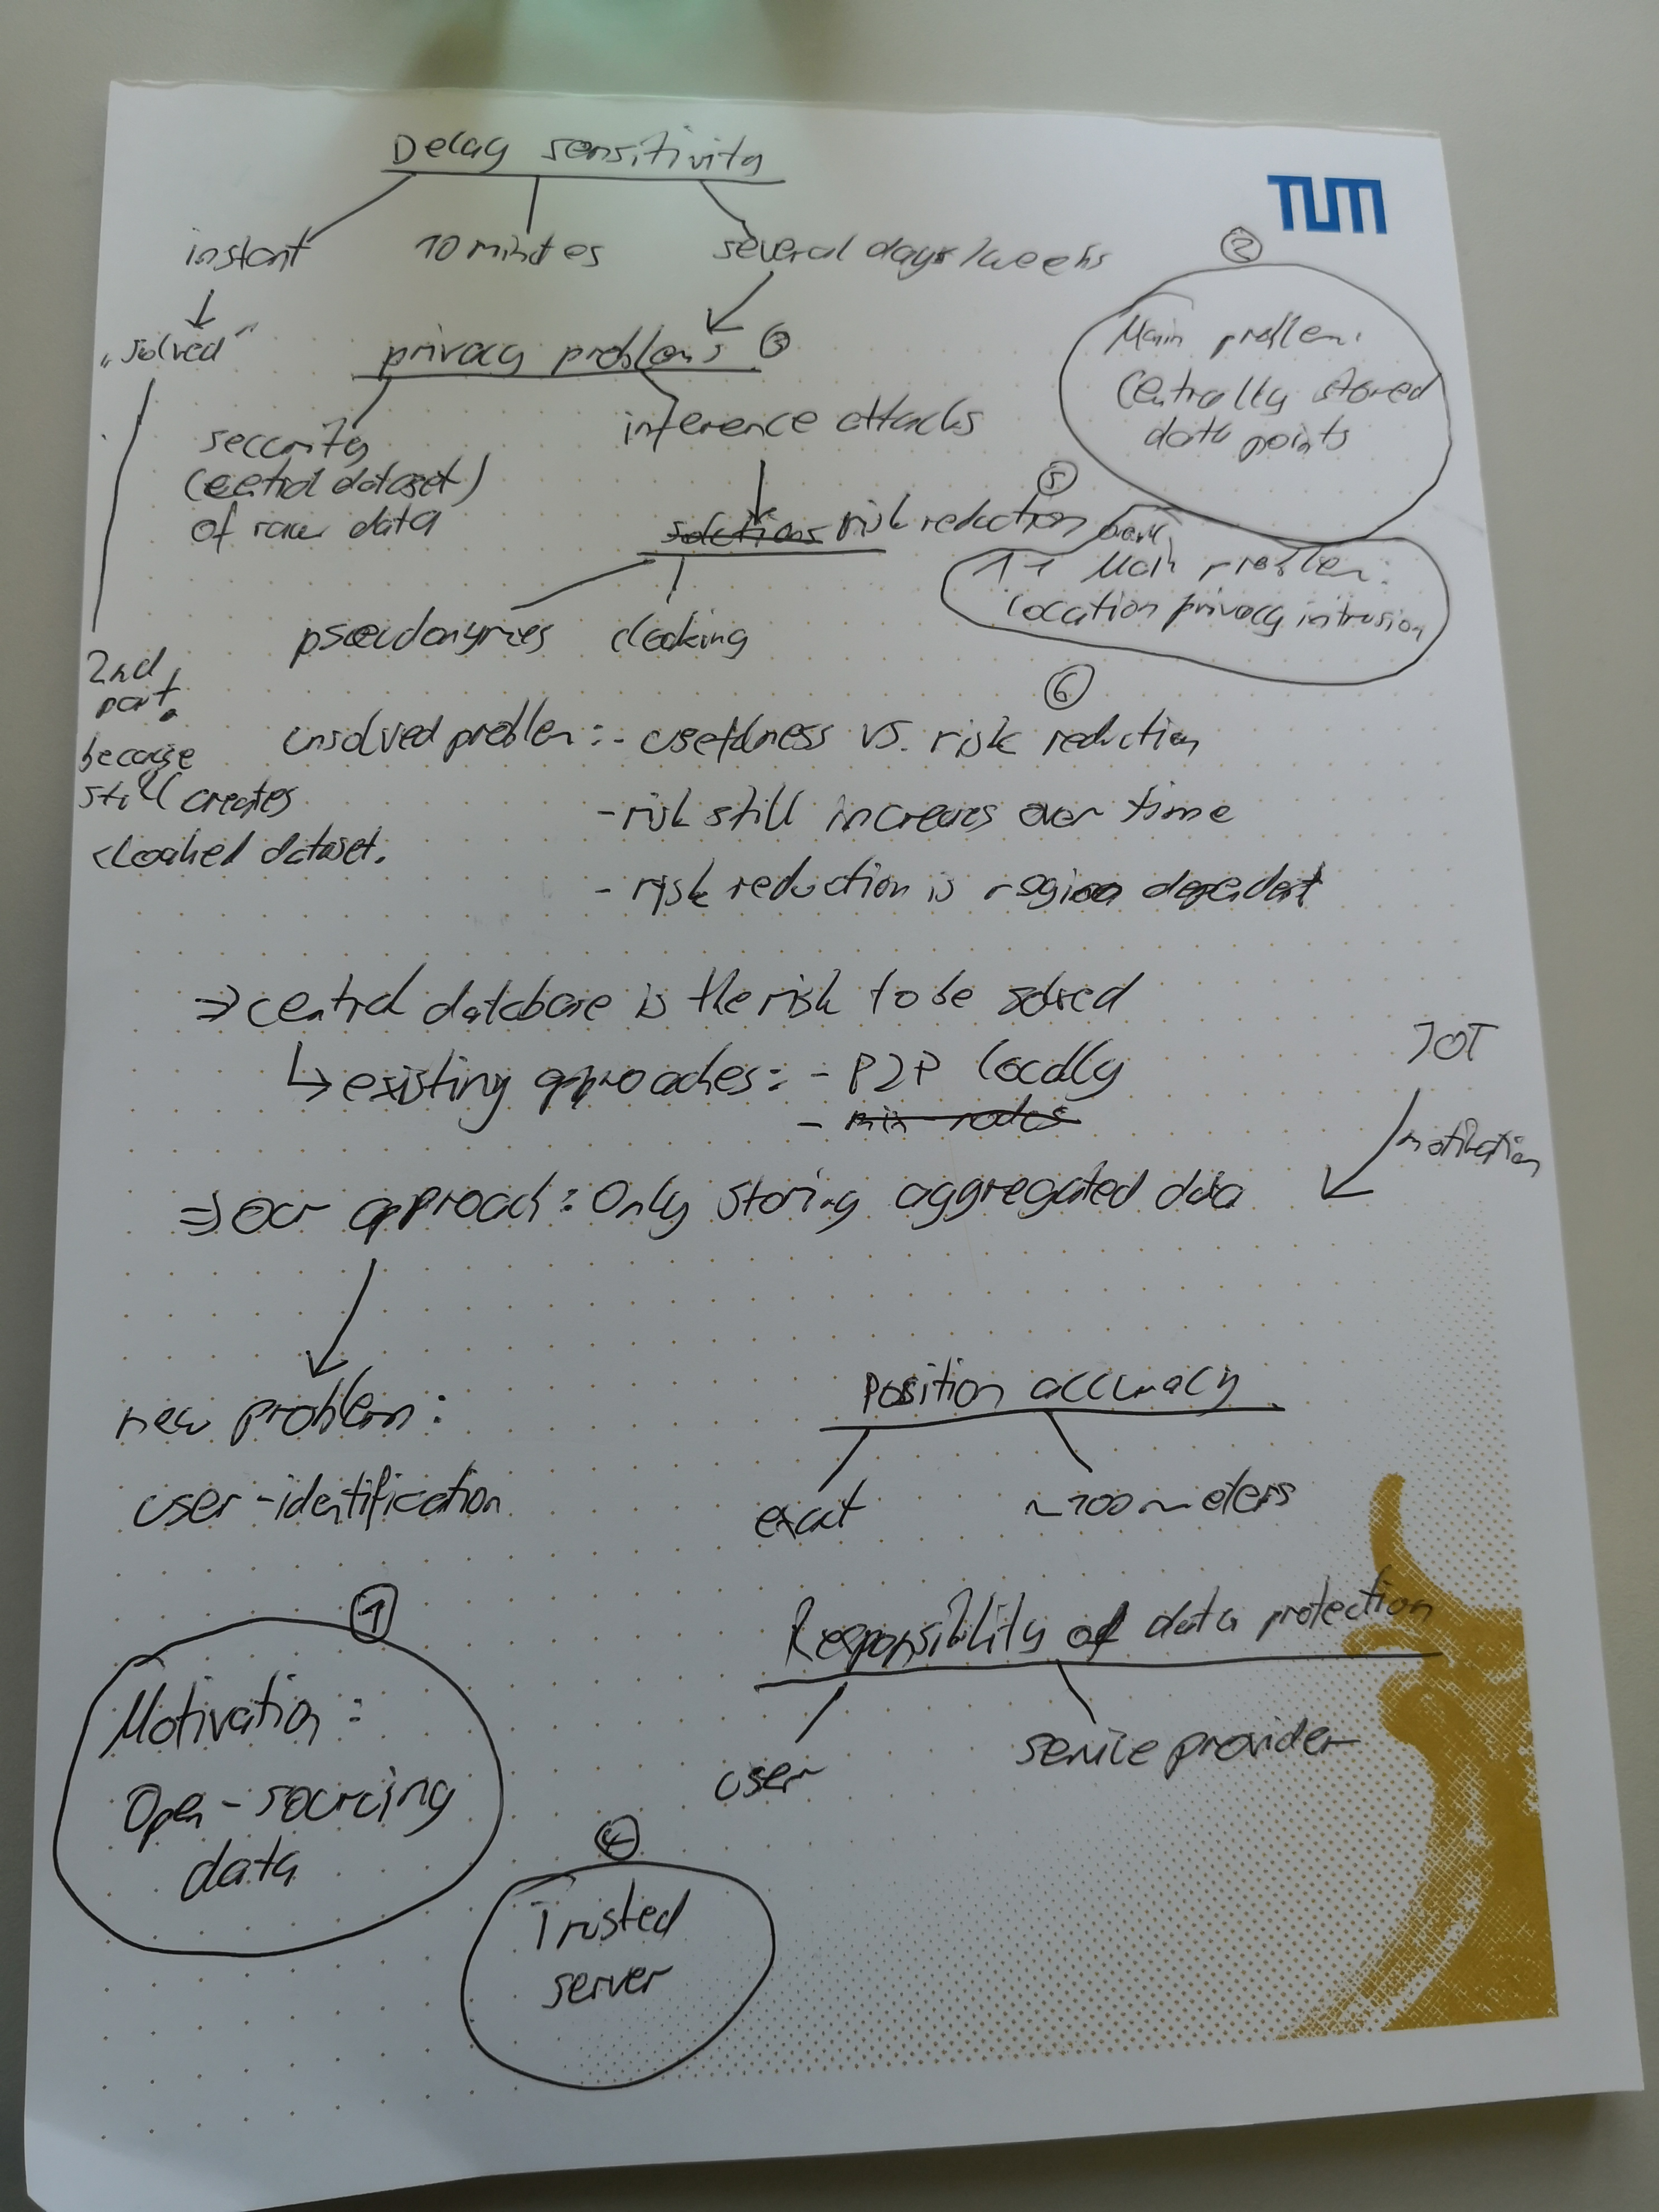
\includegraphics[width=\textwidth]{data/research-overview.jpg}
%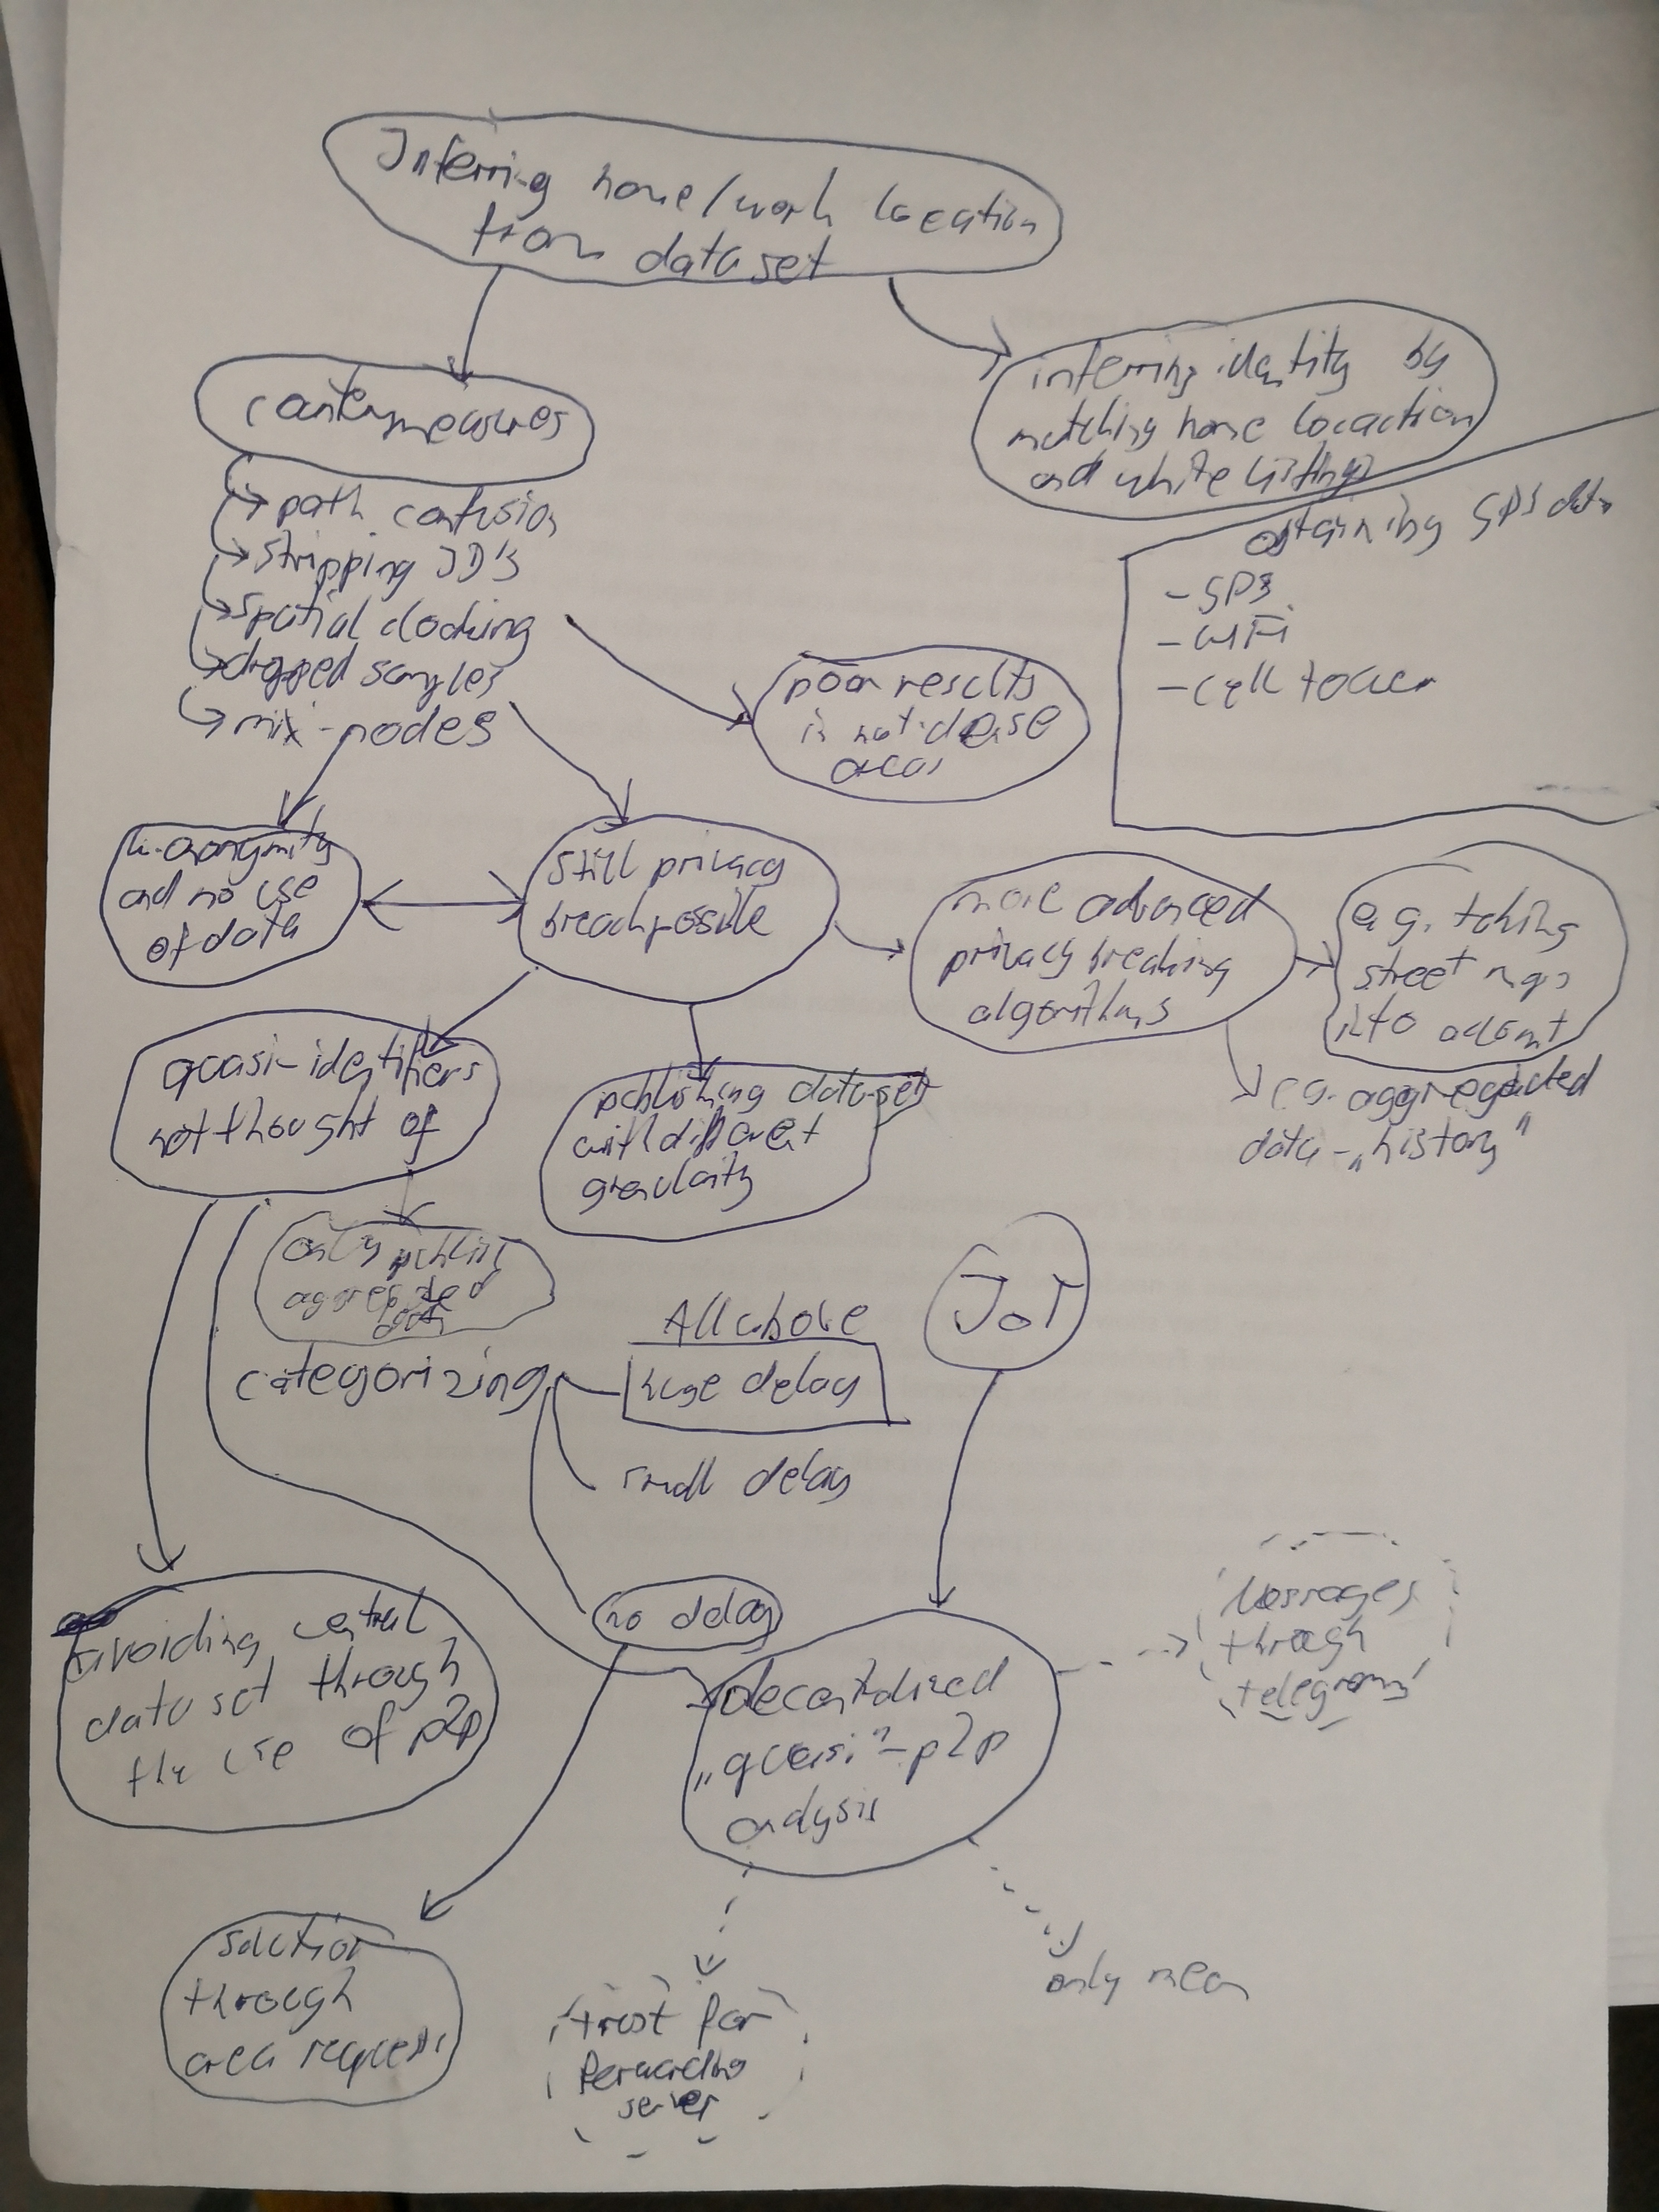
\includegraphics[width=\textwidth]{data/research-overview-2.jpg}